\section{Qt}
\begin{minipage}{17cm}
	Qt (sprich cute =süess) ist eine plattformübergreifende Programmierungsapplikation für grafische Benutzeroberflächen (GUI = Graphical User Interface).
\end{minipage}
\begin{minipage}{1.5cm}
	
\includegraphics[width=1.5cm]{images/qt_logo.jpg}
\end{minipage}

\subsection{Grundlagen zu Qt}
\begin{multicols}{2}
\subsubsection{Qt Widget}
	\begin{itemize}
		\item Qt C++ Klassenbibliothek stellt GUI-Elemente (Widget) zur Verfügung
		\item Das GUI wird als C++ Sourcefile geschrieben
	\end{itemize}
\subsubsection{Qt Quick}
	\begin{itemize}
		\item basiert auf QML , Sprache welche das Aussehen festlegt.
		\item ähnlich wie HTML
	\end{itemize}	
\end{multicols}

\subsubsection{Qt Konvention}
\begin{tabular}{|l|l|l|}
	\hline \textbf{Was} & \textbf{Beispiel} &\textbf{Konvention}\\
	\hline Qt-Modulname & "QtCore"& \textit{Qt}\\
	\hline Qt-Klassenname & "QString" & \textit{Q}\\
	\hline Qt-Variablen-,Funktionsname & "qTranslator, qDebug()"& \textit{q}\\
	\hline Qt-include & "\#include <QtGui>& \textit{ohne.h}\\
	\hline
\end{tabular}

\subsubsection{Qt Building}
\begin{itemize}
	\item qmake Makefile-Generator
	\item macht aus plattformunabhängiem Projektfile (.pro) ein plattformspezifisches Projektfile. 
	\item die gewünschte Plattform wird qmake als Option mitgegeben
	\item Bei Build-Problemen alle Dateien ausser .pro und Sourcefile löschen
\end{itemize}

\subsubsection{QObject}
%TODO QObject

\subsubsection{QWidget}
\begin{itemize}
	\item \textit{"Widget $\rightarrow$ Window Gadget / Fensterding"}
	\item Visuelles Element einer UI
	\item Toplevel Widget, alleinstehendes Fenster 
	\item Verschachtelung, in einem Widget sind weitere Widget enthalten
\end{itemize}
Objekte der Klasse QWidget sind durch Vererbung Bestandteil von Objekten der Klasse QObject. 
\begin{itemize}
	\item Alle Objekte welche von QObject abgeleitet, haben automatisches delete
	\item innerhalb eines Widget dargestellte Widgets sind \textit{"Child-Widget"}
	\item äusseres Widget ist \textit{"Parent-Widget"}
	\item Das \textit{"Parent-Widget"} übernimmt Verwaltungsfunktionen wie Memory-Management, weiterleiten von Ereignisse an \textit{"Child-Widget}, anzeigen, verstecken von Widgets etc.
\end{itemize}

\subsection{GUI-Programmierung}
Es gibt zwei grundlegende Aufgaben bei der GUI-Programmierung.\\
Das \textbf{Layout} legt Anordnung, Grösse  und Farbe fest.\\
Die \textbf{Interaktion} legt die Reaktion des Programmes auf eine Eingabe fest. \\
\newpage

\subsection{Layout}
Es gibt drei Varianten wie Widgets angeordnet werden können, absolute Positionierung, Layout Manager und GUI-Designer

\subsubsection{Absolute Positionierung}
Mittels Methoden.
\begin{multicols}{2}	
	\lstinputlisting{source/Qt/methoden.cpp}
	
	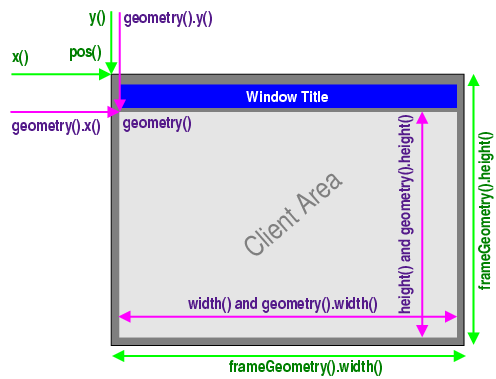
\includegraphics[width=8cm]{images/geometry.png}
\end{multicols}

\subsubsection{Layout Manager}
	\begin{tabular}{|l|l|}
		\hline \textbf{Klasse} & \textbf{Ort}\\
		\hline QVBoxLayout & Elemente vertikal\\
		\hline QHBoxLayout & Elemente horizontal\\
		\hline QGridLayout & zweidimensionales Gitter\\
		\hline QFormLayout & Elemente zeilenweise\\
		\hline QStackedLayout & aufeinandergelegt\\
		\hline
	\end{tabular}
	
\subsubsection{GUI-Designer}	
	Anordnung innerhalb eines Formulars mittels interaktiven Tools, anschliessend Umwandlung in Code. 	

\subsubsection{Top-Level-Window}
Die \textit{"Top-Level-Window"} sind Widgets welche auf der obersten Hierarchiestufe liegen. Sie haben keine \textit{"Parent-Widget"}.
Übliche Widget für \textit{"Top-Level-Window"}: 
\begin{itemize}
	\item QMainWindow $\rightarrow$ Applikations-Window (Hauptfenster)
	\item QDialog $\rightarrow$ Popup-Window für Abfragen (Wirklich löschen), Hauptanwendung bleibt blockiert
	\item QWidget $\rightarrow$ Einfaches Fenster
\end{itemize}

\subsection{Interaktion}
In Qt werden die Eingaben als SIGNALS bezeichnet und die Asugaben als SLOTS. Mittels der Funktion connect() werden die beiden miteinander verknüpft.\\
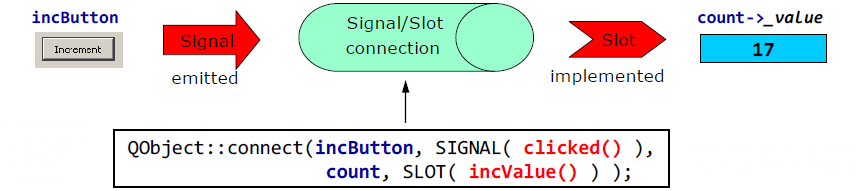
\includegraphics[width=15cm]{images/connect.png}

\begin{multicols}{3}
\subsubsection{SIGNALS}
\begin{itemize}
	\item nur deklariert, nie definiert
	\item kein Zugfriffsrecht vergeben
	\item Rückgabetyp immer void
\end{itemize}

\subsubsection{SLOTS}
\begin{itemize}
	\item deklariert und definiert
	\item oftmals Memberfunktion, auch normal abrufbar
	\item Zugriffsrechte
\end{itemize}

\subsubsection{connect}
\begin{itemize}
	\item Verbindungsfunktion zwischen Input und Output
	\item ein Signal zu mehreren Slots
	\item mehrere Signale zu einem Slot
\end{itemize}
\end{multicols}

\vspace{0.5pt}
\textbf{Beispiele connect-Funktion}
\lstinputlisting{source/Qt/connect.cpp}

\subsection{Zeichnen und Malen}
\subsubsection{QPainter}
Der Maler mit Mal-,\& Zeichenwerkzeugen.\\

\begin{tabular}{|l|l|}
	\hline \textbf{Klasse} & \textbf{Werkzeug}\\
	\hline QPen & Zeichenstift\\
	\hline QBrush & Pinsel\\
	\hline QFont & Schriftart\\
	\hline draw & Formen malen\\
	\hline
\end{tabular}

\subsubsection{QPaintDevice}
Oberfläche wo darauf gezeichnet \& gemalt werden kann
QPainter-Objekte zeigen auf QPaintDevice-Objekte. QPaintDevice ist eine abstrakte Basisklasse welche nicht von QObject abgeleitet ist und daher kein automatisches delete.\\

\begin{tabular}{|l|l|}
	\hline \textbf{Klasse} & \textbf{Funktion}\\
	\hline QWidget & -\\
	\hline QImage & Änderung Pixel\\
	\hline QPixmap & Off-Screen zeichnen, Ausgabe Bildschirm\\
	\hline QBitmap & monochrom\\
	\hline QPagedPaintDevice & Seitenformat, Ausgabe Drucker\\
	\hline
\end{tabular}

\subsubsection{Vorgehen}
\lstinputlisting{source/Qt/qpainter.cpp}